\documentclass[a4paper]{article}     
\usepackage{amsfonts}
\usepackage{amsmath}
\usepackage{amssymb}
\usepackage{graphicx}

\begin{document}
	
	\noindent \large Auteur: Victor Pena \\
	\noindent \large Studierichting: Informatica\\
	\noindent \large Oefeningenreeks 5D nr. 7.2\\
	
	\medskip
	
	\normalsize 
	
	$\displaystyle\int_{1}^{\infty} \dfrac{1}{x^2}dx = \lim\limits_{c\to\infty} \left.-\dfrac{1}{x}\right|^{c}_{1} = \lim\limits_{c\to\infty} \left(-\dfrac{1}{c} + 1\right) = 0+1 = 1 $ \\
	
	\begin{figure}[h]
	\centering
		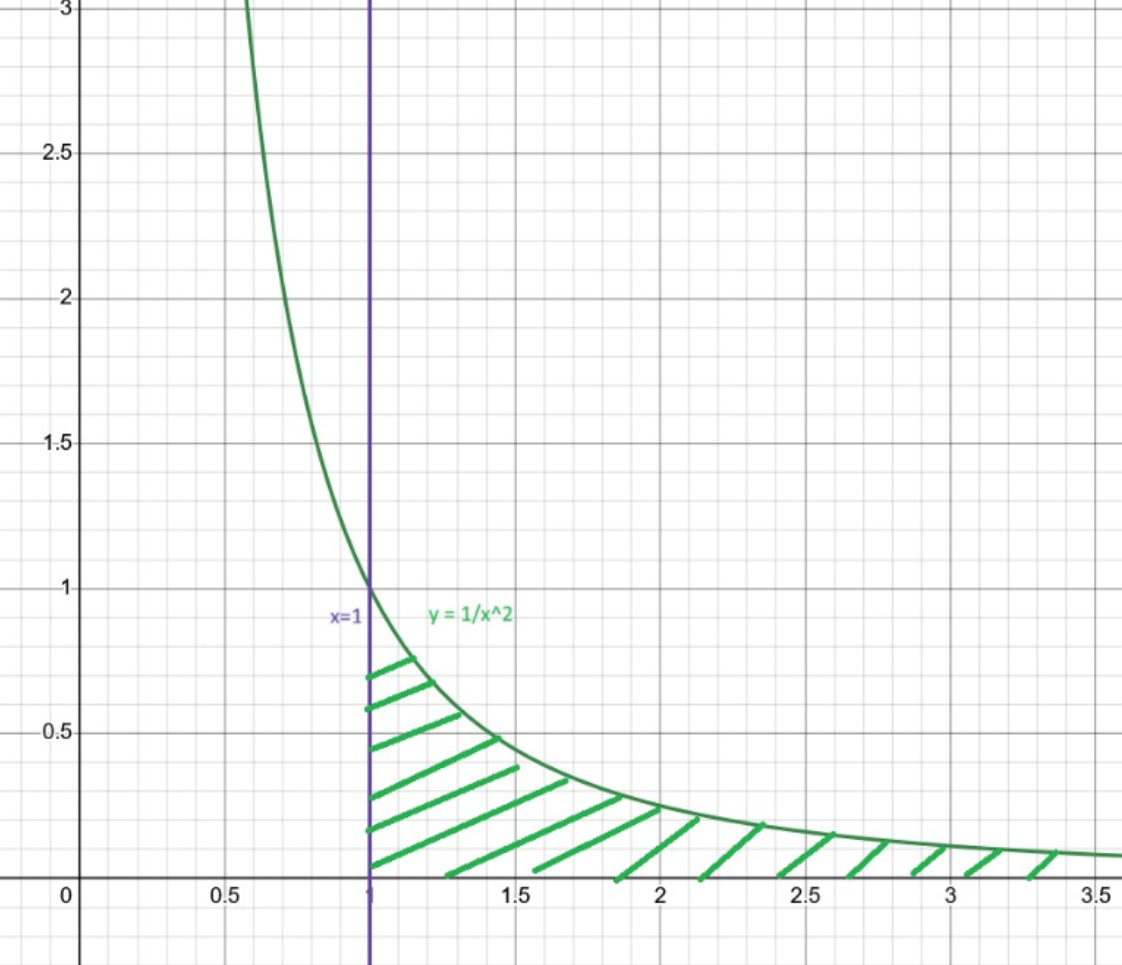
\includegraphics[width = 8cm]{5D-7.2-victor.pena.alvarado.INF.jpg}
	\end{figure}
	
	
	\begin{thebibliography}{999}
		%\bibitem{a} Referentie
	\end{thebibliography}
\end{document} 
